% 2011 年四川卷文科第 19 题：直三棱柱 ABC-A1B1C1，D 在棱 CC1 上，P 在 A1C1 的延长线上，
%   且 C1P=A1C1，AD 的延长线过 D 交于 P。
% 来源 PDF：普通高考/2011/2011四川文.pdf，SHA-256 9df4a6b69bb06bfab2f7d7ee0e7fcc50ae547f226260996d7a060c31ad14e64a。
% 原页：第 2 页（A3 三栏）第 1 栏上部，书页码 704。
% 重绘依据：照原页——顶面 ABC 可见（AC 水平），B 在左、A 在上、C 在右上；BB1 为前面的竖棱（实线），
%   CC1 实线且 D 在其中点；A1 为被遮挡的顶点，A1B1、A1C1 为虚线，B1C1 实线；
%   实线：AB、AC、BC、BB1、CC1、BD、B1C1、DP、B1P、C1P；
%   虚线：AA1、A1B1、A1C1、BA1、A1D、AD。
%   P 在 A1C1 的延长线上（C1 之外），A1C1 段虚线、C1P 段实线，照原页；原页不画顶点圆点。
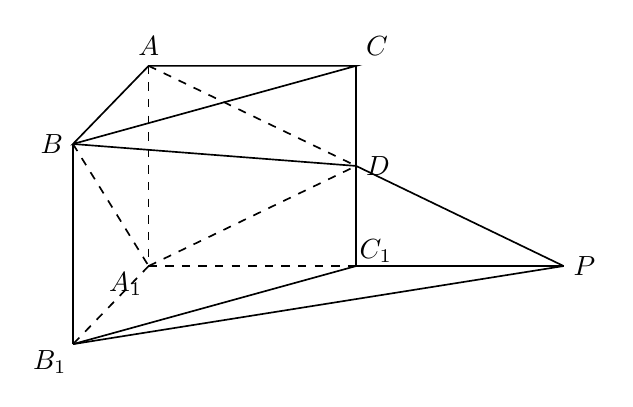
\begin{tikzpicture}[scale=0.62, >=stealth, semithick]
  \coordinate (A)  at (3.10,6.60);
  \coordinate (B)  at (1.55,5.00);
  \coordinate (C)  at (7.35,6.60);
  \coordinate (A1) at (3.10,2.50);
  \coordinate (B1) at (1.55,0.90);
  \coordinate (C1) at (7.35,2.50);
  \coordinate (D)  at (7.35,4.55);
  \coordinate (P)  at (11.60,2.50);

  % 可见的棱与辅助线（实线）
  \draw (A) -- (B) -- (C) -- cycle;
  \draw (B) -- (B1);
  \draw (C) -- (C1);
  \draw (B1) -- (C1);
  \draw (B) -- (D);
  \draw (D) -- (P);
  \draw (B1) -- (P);
  \draw (C1) -- (P);

  % 被遮挡的棱与辅助线（虚线）
  \draw[dashed] (A) -- (A1);
  \draw[dashed] (A1) -- (B1);
  \draw[dashed] (A1) -- (C1);
  \draw[dashed] (B) -- (A1);
  \draw[dashed] (A1) -- (D);
  \draw[dashed] (A) -- (D);

  \node at (A)  [above] {$A$};
  \node at (B)  [left] {$B$};
  \node at (C)  [above right] {$C$};
  \node at (A1) [below left, inner sep=2pt] {$A_1$};
  \node at (B1) [below left, inner sep=2pt] {$B_1$};
  \node at (C1) [above right, inner sep=1pt] {$C_1$};
  \node at (D)  [right] {$D$};
  \node at (P)  [right] {$P$};
\end{tikzpicture}
